\documentclass{article}

\NeedsTeXFormat{LaTeX2e}
\newcommand{\course}[1]{\newcommand{\CourseTitle}{#1}}
%\newcommand{\title}[1]{\newcommand{\PaperTitle}{#1}}

%% Common helper packages %%%%%%%%%%%%%%%%%%%%%%%%%%%%%%%%%%%%%%%%%%%%%%%%%%%%%%

\usepackage{fancyhdr}
\usepackage[usenames]{color}
\usepackage{alltt}
\usepackage[letterpaper,margin=1in]{geometry}
\usepackage{parskip}
\usepackage{xstring}
\usepackage{comment}
\usepackage{amsmath}
\usepackage{amsfonts}
\usepackage{multicol}
\usepackage{amssymb}
\usepackage{bm}
\usepackage{lmodern}
\usepackage{graphicx}
\usepackage{titling}
%\RequirePackage{utf8}
\usepackage{fancyhdr}
\usepackage{titlesec}
\usepackage{scrextend}

\graphicspath{{images/}}

\frenchspacing

%\renewcommand\@maketitle{
%  \setlength\parindent{0in}
%  \addtolength\parskip{1ex}
%  \setlength\fboxrule{.5mm}\setlength{\fboxsep}{1.2mm}
%  \newlength\courseheader
%  \setlength\courseheader\textwidth
%  \addtolength\courseheader{-4mm}
%  \begin{center}
%  \framebox{\parbox\courseheader{\large
%  \CourseTitle\hfill Spring 2016\\
%  Tennyson T Bardwell \hfill \@title}}
%  \end{center}
%  \bigskip
%}
%
%\newcommand{\makecover}{
%  \vspace*{.45\textheight}
%  \thispagestyle{empty}
%  \begin{center}
%  {
%  \huge
%  \textbf{\@title\\}
%  \noindent\rule[0.5ex]{\linewidth}{1pt}
%  \large
%  Tennyson T Bardwell\\
%  \CourseTitle\\
%  Spring 2016\\
%  }
%  \pagebreak
%  \end{center}
%}



\usepackage{hyperref}
\usepackage{float}
% \usepackage{media9}


\newcommand{\CoverAuthor}{
  Tennyson T \textsc{Bardwell} (ttb33)\\
  Quinn \textsc{Halpin} (qmh4)\\
  Sitar \textsc{Harel} (sh927)\\
  % Alex \textsc{Ozer} (aso26)\\
}
\newcommand{\HeaderAuthor}{Powder Shell}
\newcommand{\Title}{Powder Shell\\\vspace{.5 em}Final Design Document}
\newcommand{\CouseCode}{CS 3110}
\newcommand{\CouseName}{Data Structures and Functional Programming}
\newcommand{\ProfessorName}{Michael \textsc{Clarkson}}

\pagestyle{fancy}
\lhead{\HeaderAuthor}

\titleformat{\section}
  {\normalfont\LARGE\bfseries}
  {\thesection}{1em}{}[{\titlerule[0.8pt]}]


\begin{document}
\sloppy

%%%%%%%%%%%%%%%%%%%%%%%%%%%%%%%%%%%%%%%%%
% University Assignment Title Page 
% LaTeX Template
% Version 1.0 (27/12/12)
%
% This template has been downloaded from:
% http://www.LaTeXTemplates.com
%
% Original author:
% WikiBooks (http://en.wikibooks.org/wiki/LaTeX/Title_Creation)
%
% License:
% CC BY-NC-SA 3.0 (http://creativecommons.org/licenses/by-nc-sa/3.0/)
% 
% Instructions for using this template:
% This title page is capable of being compiled as is. This is not useful for 
% including it in another document. To do this, you have two options: 
%
% 1) Copy/paste everything between \begin{document} and \end{document} 
% starting at \begin{titlepage} and paste this into another LaTeX file where you 
% want your title page.
% OR
% 2) Remove everything outside the \begin{titlepage} and \end{titlepage} and 
% move this file to the same directory as the LaTeX file you wish to add it to. 
% Then add \input{./title_page_1.tex} to your LaTeX file where you want your
% title page.
%
%%%%%%%%%%%%%%%%%%%%%%%%%%%%%%%%%%%%%%%%%

%----------------------------------------------------------------------------------------
%	PACKAGES AND OTHER DOCUMENT CONFIGURATIONS
%----------------------------------------------------------------------------------------

% \documentclass[12pt]{article}

% \begin{document}

\begin{titlepage}

\newcommand{\HRule}{\rule{\linewidth}{0.5mm}} % Defines a new command for the horizontal lines, change thickness here

\center % Center everything on the page
 
%----------------------------------------------------------------------------------------
%	HEADING SECTIONS
%----------------------------------------------------------------------------------------

\textsc{\LARGE Cornell University}\\[1.5cm] % Name of your university/college
\textsc{\Large \CouseCode}\\[0.5cm] % Major heading such as course name
\textsc{\large \CouseName}\\[0.5cm] % Minor heading such as course title

%----------------------------------------------------------------------------------------
%	TITLE SECTION
%----------------------------------------------------------------------------------------

\HRule \\[0.4cm]
{ \huge \bfseries \Title}\\[0.4cm] % Title of your document
\HRule \\[1.5cm]
 
%----------------------------------------------------------------------------------------
%	AUTHOR SECTION
%----------------------------------------------------------------------------------------

\begin{minipage}{0.4\textwidth}
\begin{flushleft} \large
\emph{Authors:}\\ \CoverAuthor
\end{flushleft}
\end{minipage}
~
\begin{minipage}{0.4\textwidth}
\begin{flushright} \large
\emph{Professor:} \\ \ProfessorName
\end{flushright}
\end{minipage}\\[4cm]

% If you don't want a supervisor, uncomment the two lines below and remove the section above
%\Large \emph{Author:}\\
%John \textsc{Smith}\\[3cm] % Your name

%----------------------------------------------------------------------------------------
%	DATE SECTION
%----------------------------------------------------------------------------------------

{\large \today}\\[3cm] % Date, change the \today to a set date if you want to be precise

%----------------------------------------------------------------------------------------
%	LOGO SECTION
%----------------------------------------------------------------------------------------


\includegraphics[width=3cm]{images/cu.png}\\[1cm] % Include a department/university logo - this will require the graphicx package
 
%----------------------------------------------------------------------------------------

\vfill % Fill the rest of the page with whitespace

\end{titlepage}
% \end{document}


\section{System description}

\textbf{Summary:} Implement an ASCII version of the beloved powder game that runs in the terminal. See \url{http://dan-ball.jp/en/javagame/dust/} for an example.

\subsection{Key Features}
\begin{enumerate}
  \item A full, working, implementation of the powder game inside of a terminal.
  \item Elements include: sand, water, ice, stone, glass, lava, steam, plant, fire, torch, black hole, water spout, oil, acid, bomb, and stem cell.
  \item Accepts mouse interaction and keyboard shortcuts as forms of user interaction to add/remove element and select element type to add.
  \item Implement a json config file to define element's properties. 
  \item Include a saving/loading to/from file.
\end{enumerate}

\subsection{Description}
The powder game first appeared on dan-ball.jp at \url{http://dan-ball.jp/en/javagame/dust/} and has since been copied, ported, and expanded many times over. However, to this day, there exists no terminal based, ASCII-only, playable version of this beloved game---until now. We have corrected this atrocity.

Our implementation is quick enough to be played on low end machines, flexible enough to adapt to different screen sizes, and intuitive enough so that even a new player can play effectively. 

This implementation of the ASCII powder game involves minimal physics and no velocity vectors. We save the state of the pixel location as a mutable 2D array. The engine outputs the next state of the game based off the current state and on a user's selected element and mouse clicks. All the materials have their own Json file with a list of traits. This makes adding a new element simple. For example, sand can be defined by traits such as color = yellow and movement = slightly viscous. Some elements will also be able to respond to other elements for example, ice will turn all water pixels into ice. A game can be saved and stored to a file.

\section{Architecture}
TODO

All modules will communicate with the main module only (with the exception of their
peripherals such as Lamda Term or the file system). This allows only one module, the
main module, to be solely concerned with the coordination of the roles of different
modules. See figure \ref{fig:com} for the communication and interfaces between modules.
Since our architecture makes it difficult to see the flow of logic, data, and state during
runtime we have also provided figure \ref{fig:run} which shows the flow of information
throughout our program at runtime.

\begin{figure}[H]
  \caption{Communications between modules}
  \label{fig:com}
  \vspace{3em}
  \center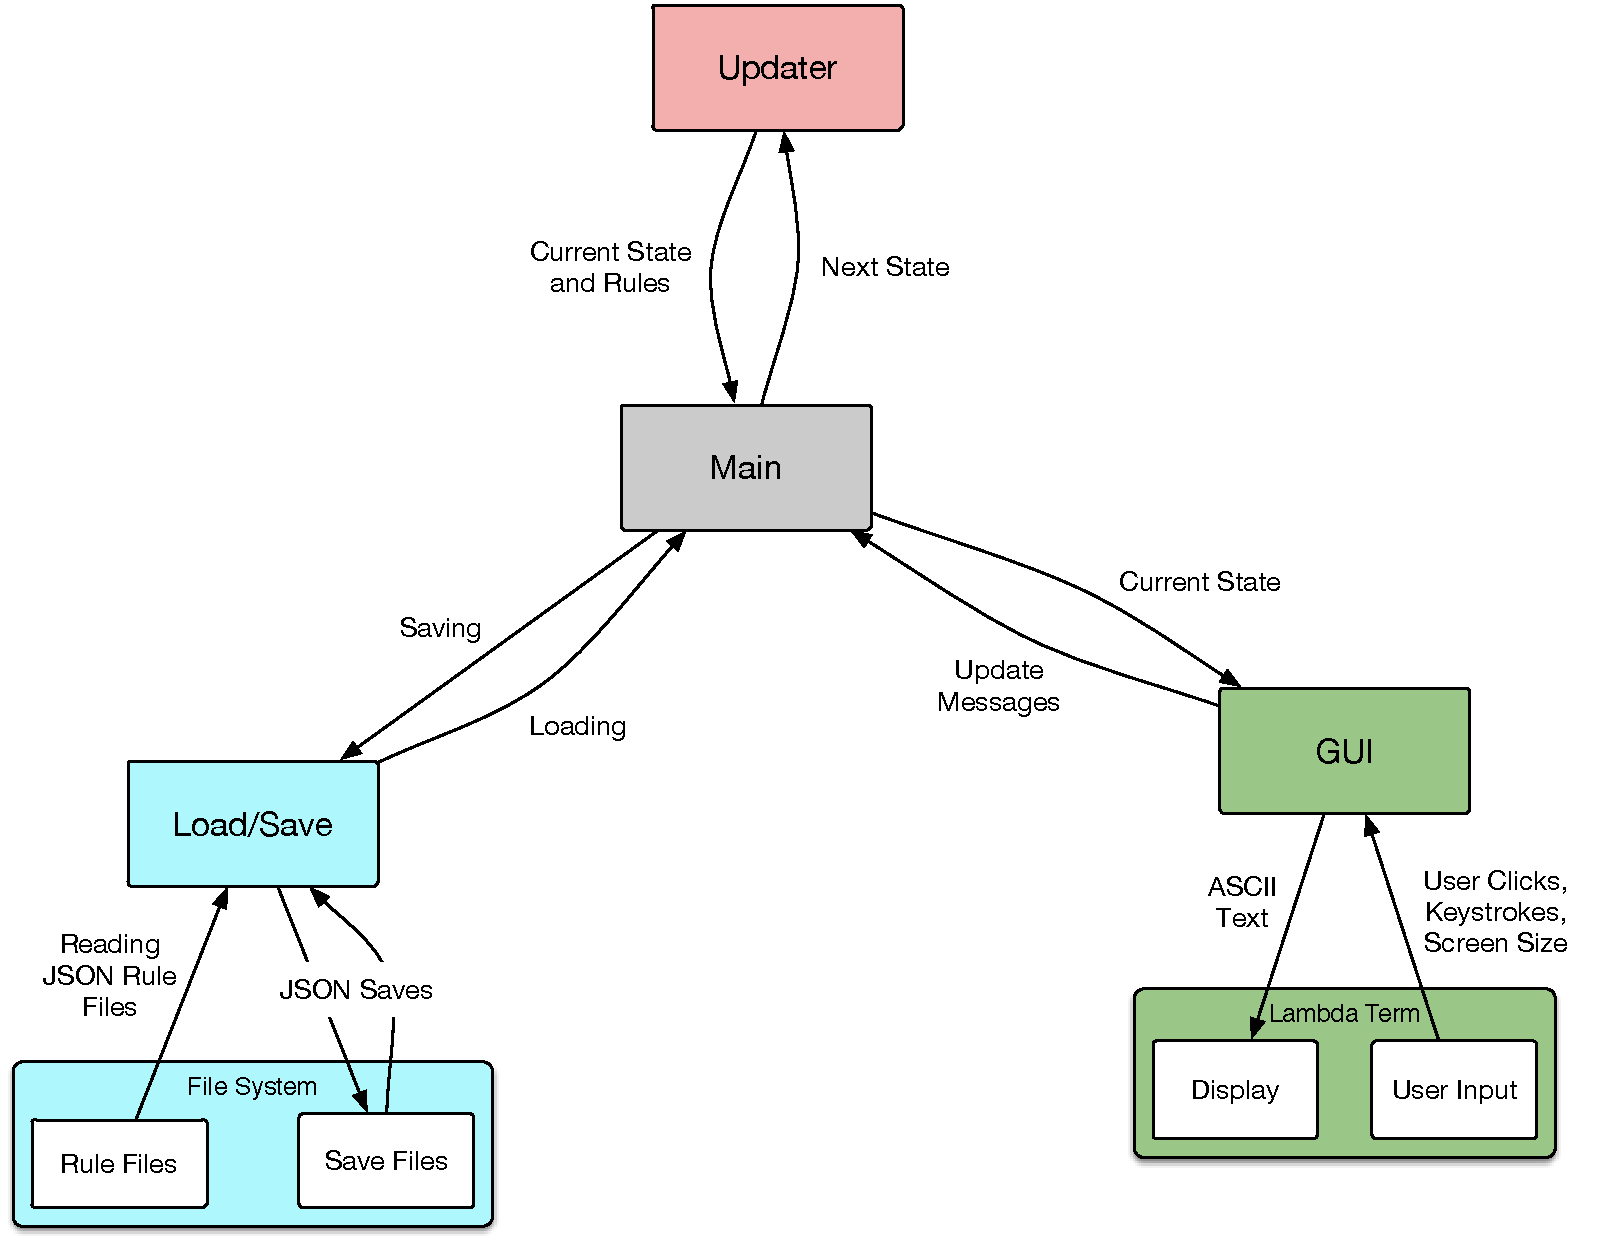
\includegraphics[width=0.7\textwidth]{images/communications}
\end{figure}

\begin{figure}[H]
  \caption{Runtime Flow of Information}
  \label{fig:run}
  \vspace{3em}
  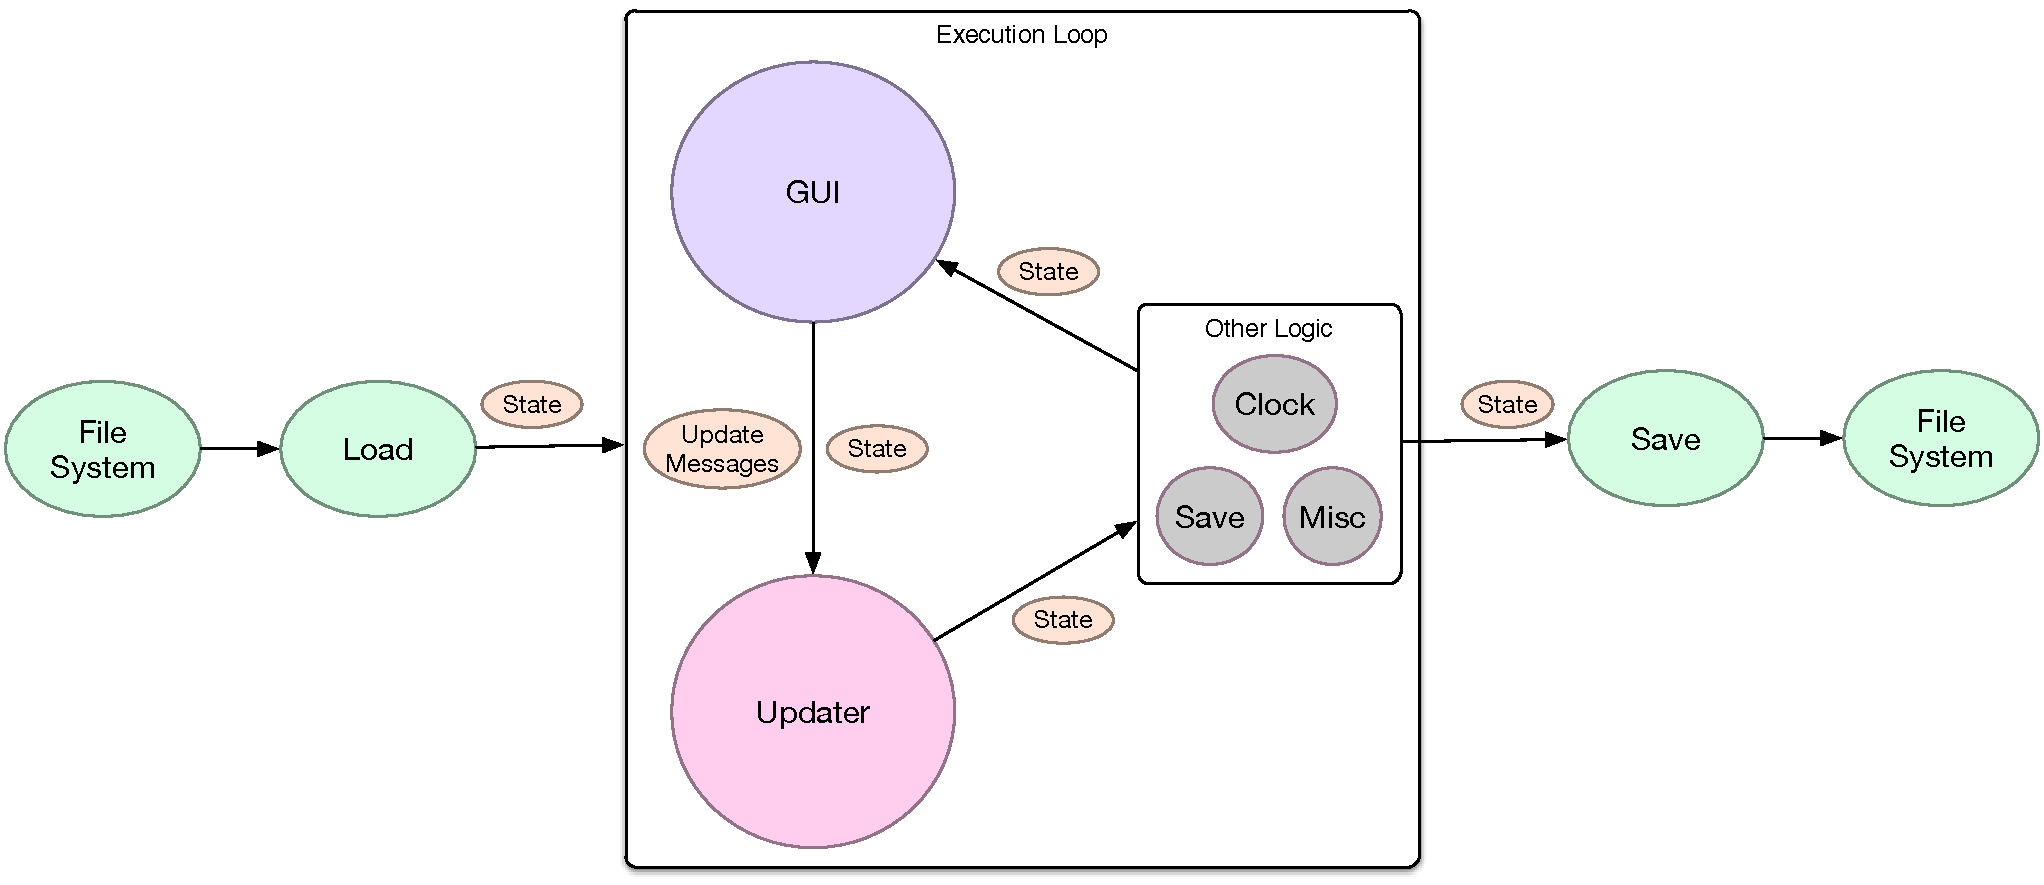
\includegraphics[width=\textwidth]{images/runtime_order}
\end{figure}

\section{System design}
TODO

Each module is completely separate except for 1) main, which manages the coordination
of the whole program and 2) the sharing of data objects between modules. This can be
seen below in figure \ref{fig:dep}.

\begin{figure}[H]
  \caption{Module Dependency Diagram}
  \label{fig:dep}
  \vspace{3em}
  \center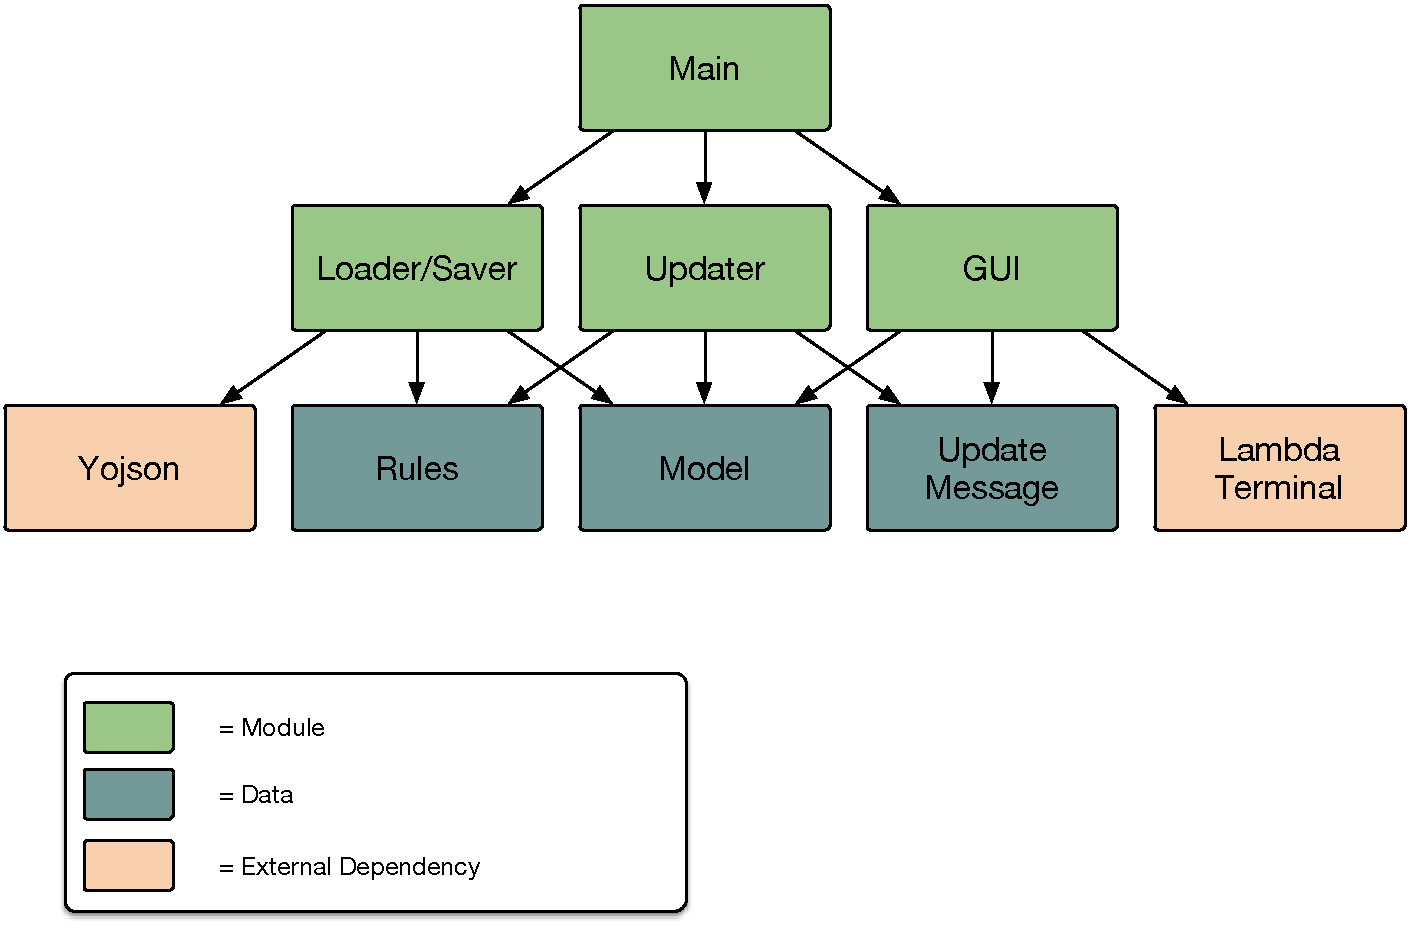
\includegraphics[width=0.8\textwidth]{images/dependencies}
\end{figure}

\subsection{Modules}
TODO

\begin{description}
  \item[main:] coordinates all other modules, passing them the required state/message updates/rules for them to function and ordering the actions of other modules
  \item[load/save:] loads rules and states from file to memory representations and reverses the process to save states (never saves rules)
  \item[gui:] displays the current state to the user using ASCII text through the terminal, also records user interactions and packages them as model updates
  \item[updater:] manages all changes to the state from updating frame to frame and by processing model updates
  \item[clock:] prevents the game from running pass a set frame rate
\end{description}

\subsection{Updater Logic}
The updater can take a single, instantanous state and a set of rules and produces the state at
the next time step. How this could work is demonstrated below for the elements sand and water:

Sand falls to the ground through simple rules:
\begin{enumerate}
  \item If the space immediately below it is empty then it will move to that space.
  \item If a space below it and immediately to the right or left is empty than it moves
    to one of those spaces (possibly picked randomly).
\end{enumerate}
See an example below in figure \ref{fig:sand}.

\begin{figure}[H]
  \caption{The falling of sand}
  \label{fig:sand}
  \vspace{3em}
  \center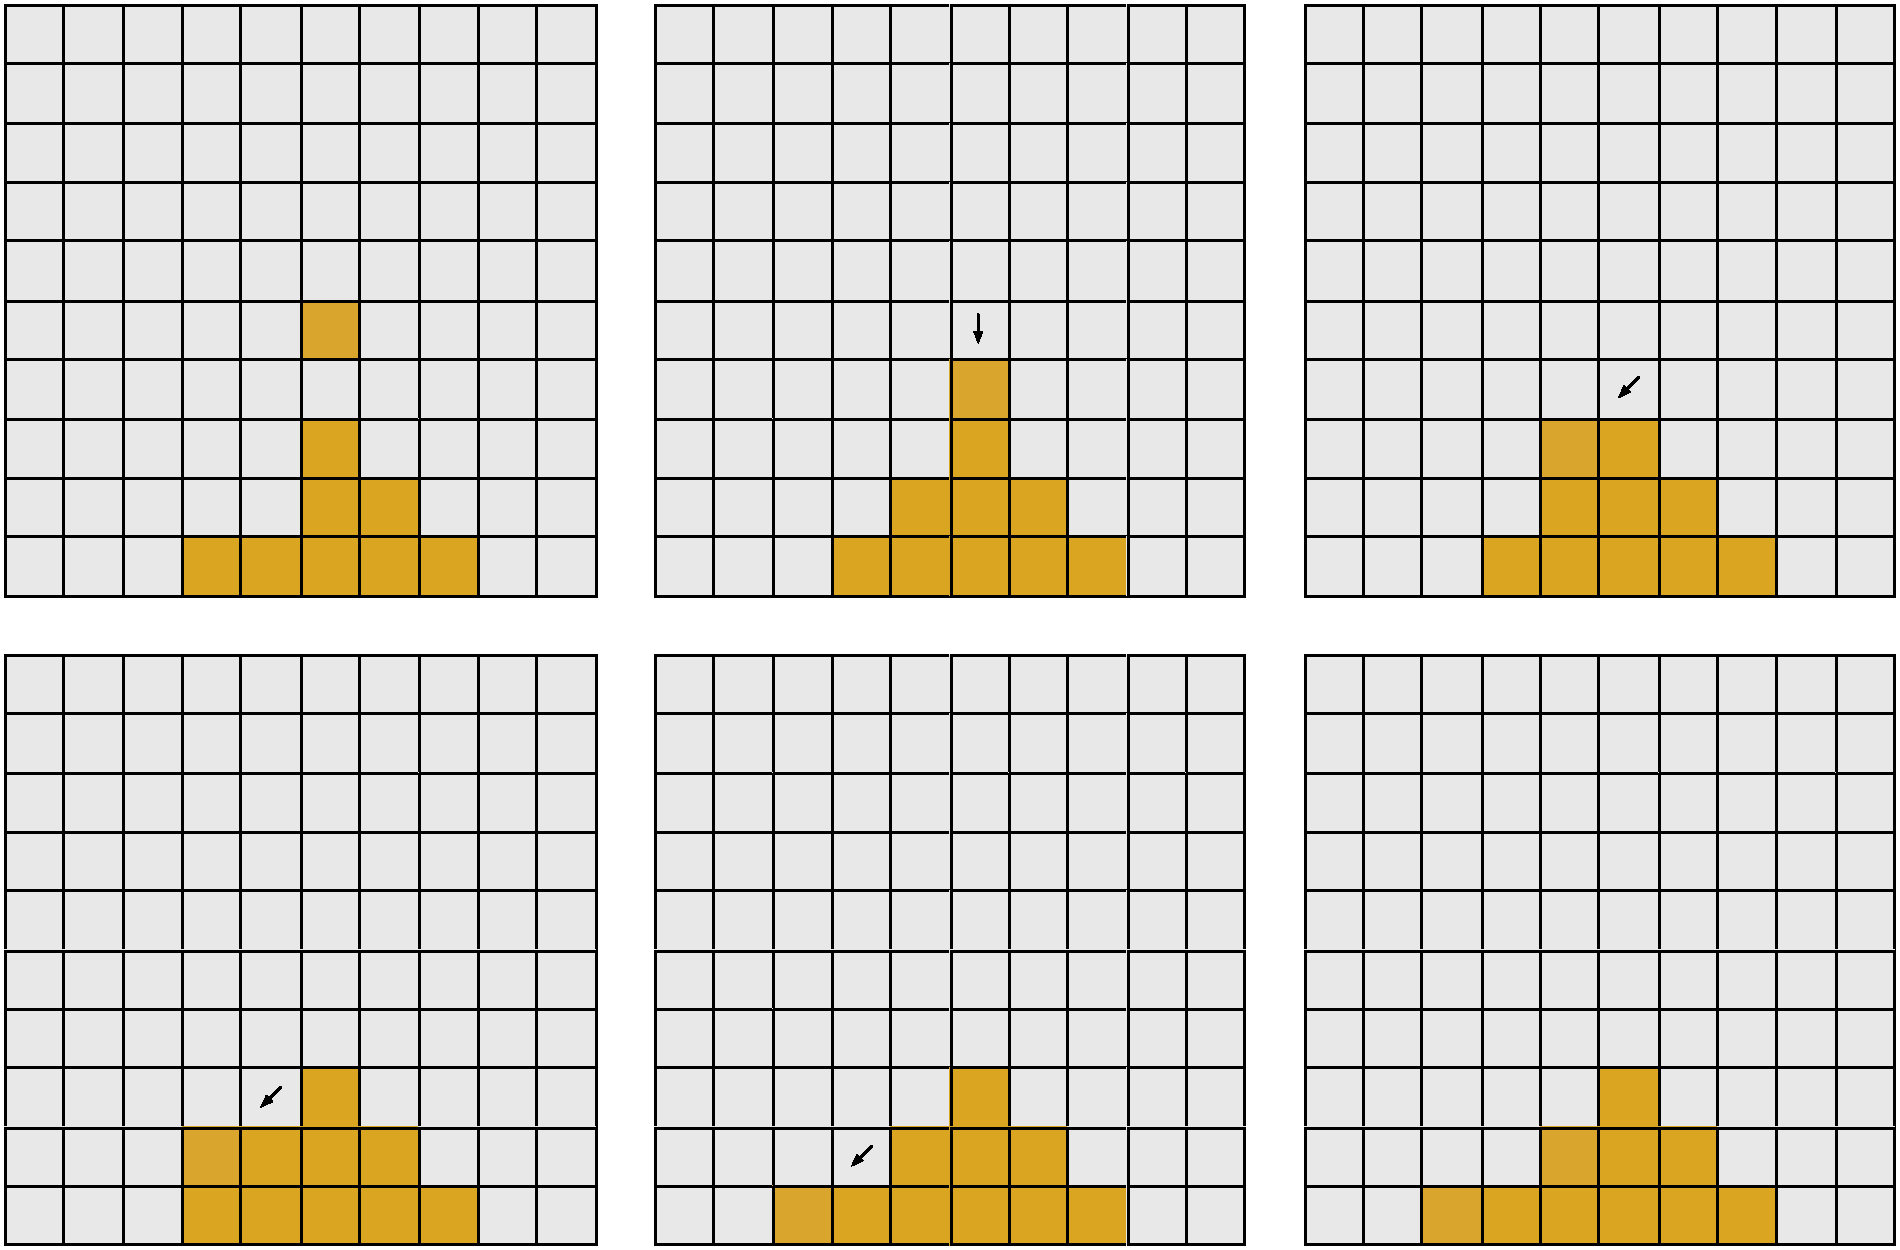
\includegraphics[width=0.9\textwidth]{images/grid_sand}
\end{figure}

Water merely introduces another rule:
\begin{enumerate}
  \item[3] If the space immediately next to it on either side is empty then it has a chance
    of moving to that space (randomly picking if both are empty).
\end{enumerate}
See an example below in figure \ref{fig:water}.

\begin{figure}[H]
  \caption{The falling of sand}
  \label{fig:water}
  \vspace{3em}
  \center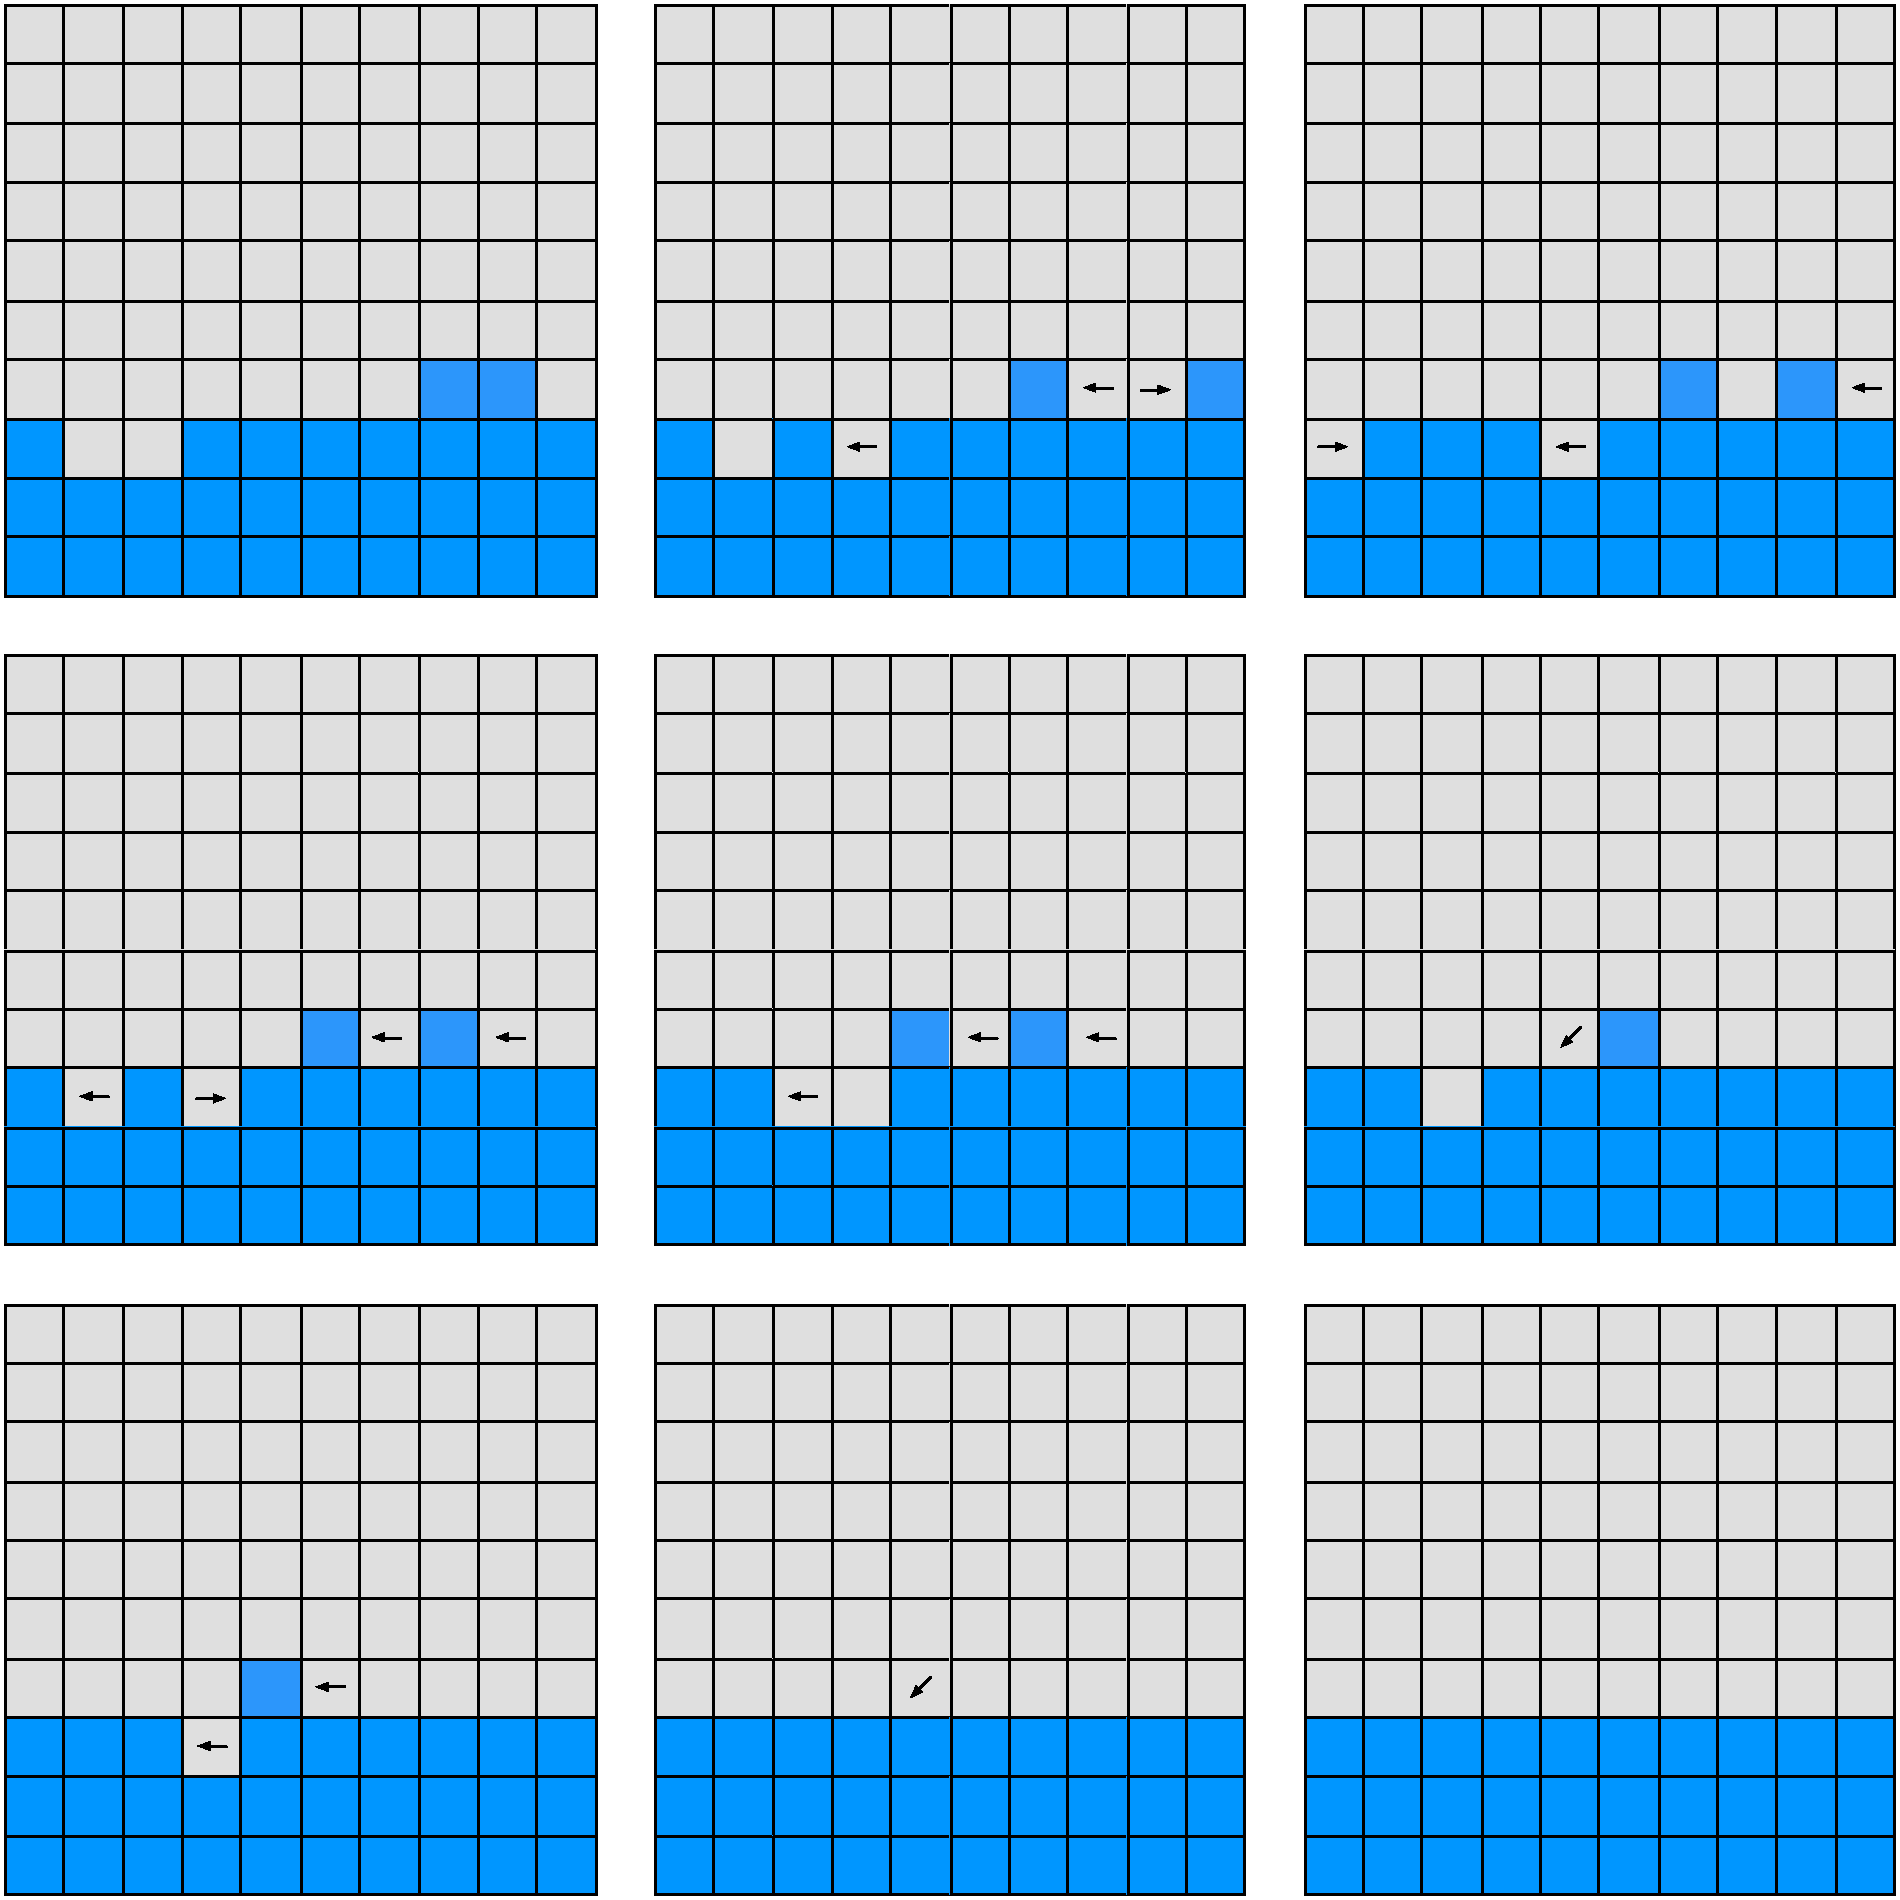
\includegraphics[width=0.9\textwidth]{images/grid_water}
\end{figure}

\section{Data}
The grid maintain the location of particles and the name of the particle at that location. The rules are held seperately in its own json file and maintains characteristics such as density, iteractions, color, change, destroy, and grow. The grid is represented as a (location_t * particle_t) array array, where location_t is type int*int and particle_t is of type {name = string}. 

Rules is an assoc list with the name of an elem associated with an elem_rules. Elem_rules record consits of 
a bunch of tuples, records, and lists, that are associated with an element. Something like color of an element, 
density of an element, and transforming that elemnent to a different element with a certain probability would
all belong under Elem_rules.

\section{External Dependencies}
We used Lambda-Term (\url{https://github.com/diml/lambda-term}), an open source library that allows us to interface with the terminal, not just through keyboard input, but also with the mouse. We also used Yojson for parsing JSON data from our rules file and from save files.

\section{Testing}
We have tested our system in three ways. First, we have done black box and glass box testing based on our interface files to test each function in Model interface file and File Manager interface file. Second, we have
personally spent hours playing the game to test the GUI and have given the game to other people to test. 

We have been holding our team accountable be checking everyone meets their test plan at our bi-weekly meeting and scan over the test suite. Of course, all the code and test suites for each module will be available on the GitHub.

\section{Division Of Labor}
Tennyson designed rules, updater, and rules json parsing. 

Quinn implemented the interface for model, writing the grid to a json file, 
reading a json file to a grid, and wrote test cases for model and filemanager. 
She spent some time making json parsing to a grid more efficient so that only the 
locations that are not empty show up in the json file. She did 50 hours of work.

Sitar implemented GUI which involved drawing particles to the terminal and 
managing the entire user interface. He spent over 70 hours deciphering the quirks 
of lambda-term and figuring out how to get the best user experience out of the terminal.
Sitar also implemented the asynchronous logic of main.ml and designed many of 
the elements in the rules JSON.


\begin{description}
  \item[Tennyson T Bardwell (ttb33):]
    Implemented the majority of the updater's logic which increments from one step to the next and applied user input to the grid. Also, defined the initial rules for sand and water, implementing the JSON structure for the rules of these elements, the in memory representation, and the parsing of the JSON. Wrote many updater test cases. Estimated hours of work: 40.
  \item[Quinn Halpin (qmh4):]
  \item[Sitar Harel (sh927):]
\end{description}

\end{document}

